
%%% Local Variables:
%%% mode: latex
%%% TeX-master: t
%%% End:

\chapter{重点枢纽行人微观模型建设}
行人微观仿真模型旨在对微观交通枢纽内部的行人交通组织方案进行仿真
评价与优化; 结合枢纽内部现状或者规划行人步行设施情况,利用 Legion 软件
对人流情况进行仿真,并结合实际观察结果对仿真模型和参数进行调整, 具体工
作包括:

\begin{cit}
\item 建立基于微观行人仿真的技术流程;
\item 形成仿真成果数据分析图和行人仿真视频
\item 通过交通仿真,对行人交通组织方案进行评价,为相应的枢纽详细规划提供支持。
\end{cit}

\section{交通枢纽概况}
\subsection{大运枢纽站}
在城市轨道交通建设过程中,交通枢纽详细规划项目对于内部人流的交通组
织要求越来越高, 因此迫切需要对重点交通枢纽建立室内行人微观仿真模型, 将
模型与方案相结合, 用模型辅助方案设计。 结合 2017 年深圳市重点交通枢纽详
细规划项目, 本项目新建大运枢纽微观行人仿真模型。

深圳市 2、 14、 16 号线已列入四期建设规划并正式开工建设,急需开展大运
站枢纽交通详细规划工作,为枢纽工程设计提供依据。如图\ref{fig:chp06_大运枢纽详细规划项目的研究范围和规划范围}所示,
详细规划范围东至亲河路,南至机荷高速、惠盐高速,西至红棉路,北至黄阁南路、爱南路,
面积约 140公顷; 规划范围东至红棉路,南至荷韵路,西至龙岗大道,北至荷风路,面积约15.6 公顷。

\begin{figure}[!ht]
  \centering
  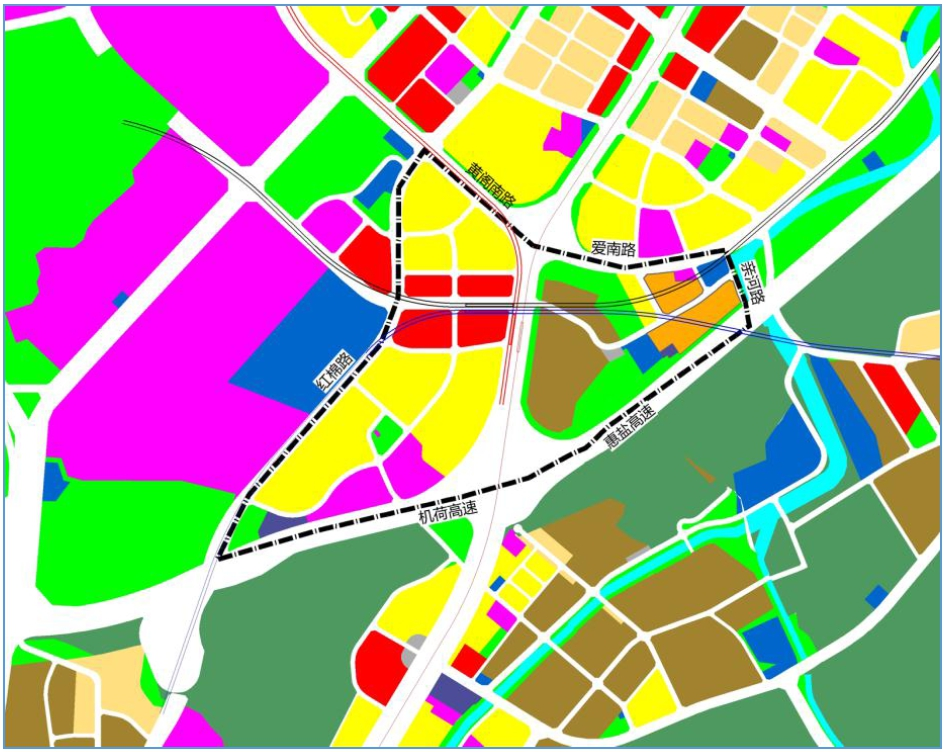
\includegraphics[width=0.9\textwidth]{chp06_大运枢纽详细规划项目的研究范围和规划范围.jpg}
  \caption{大运枢纽详细规划项目的研究范围和规划范围\label{fig:chp06_大运枢纽详细规划项目的研究范围和规划范围} }
\end{figure}

大运站在远期规划中将是 14、 16 和 33 号线的站点, 同时兼具城际轨道线和
市内轨道线双重职能。 考虑到大运站未来重要的枢纽作用, 因此在宏观轨道客流
评估阶段预测未来高峰客流将达到 55 万人次; 而且多线换乘导致站内结构、 行
人通道设计和流向组织都非常复杂,室内包括上下三层共六层的建筑设计。图\ref{fig:chp06_大运枢纽建筑竖向布局}
是枢纽的竖向布局图以及行人步行流向。

\begin{figure}[!ht]
  \centering
  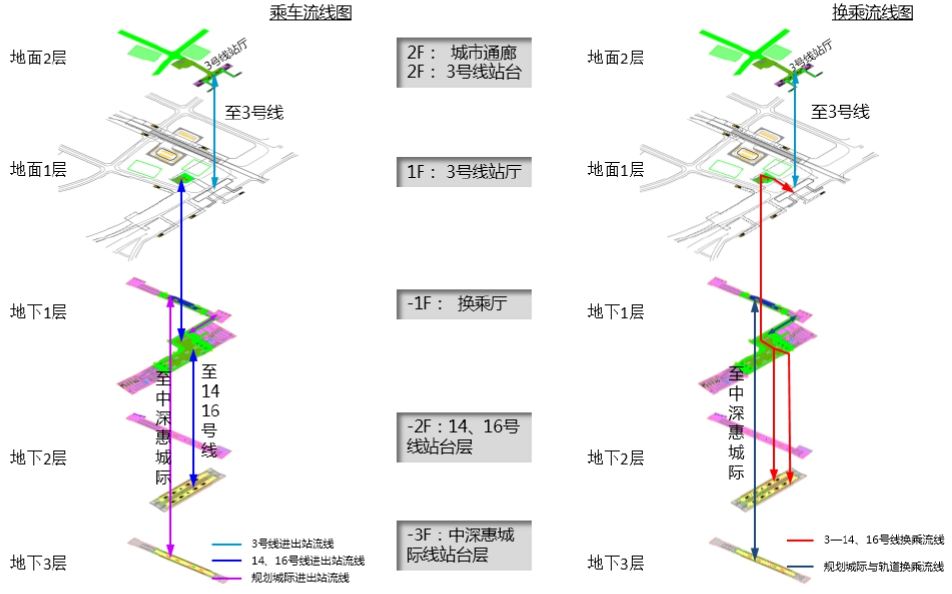
\includegraphics[width=\textwidth]{chp06_大运枢纽建筑竖向布局.jpg}
  \caption{大运枢纽建筑竖向布局\label{fig:chp06_大运枢纽建筑竖向布局} }
\end{figure}

\clearpage

\subsection{高新园站}
高新园站是 1 号线的一个普通站, 上下共两层。 但是, 由于高新园区近年来
的高密度开发, 该站已经成为深圳轨道站点中高峰客流量最大的站之一, 三期开
通后的日均高峰小时客流量高达 2.4 万人次,其中晚高峰进站量 1.5 万人次,出
站量 0.17 万人次,呈现严重的潮汐现象。 因此, 本项目对高新园站的人流进行
了仿真, 重点分析站内人流饱和度。

\section{关键技术}
通过微观行人仿真模型,可依据交通枢纽行人组织方案和室内建筑平面图,
形象生动的展示枢纽内部的行人步行交通情况,发现潜在的拥挤区域和形成原因,
并有效地对各种方案进行评价和对比。因此, 从技术层面, 基于 Legion 行人仿
真软件的仿真建模需要的基础数据至少包括: 建筑内部平面设计图、行人步行设
施设计方案; 另外,针对行人步行特征、 排队特征、进出口 OD 人流量等需要分
别设计模型参数, 最后再根据输入数据运行模型, 制作行人仿真视频录像和数据
分析图。 具体的流程如下图所示。

\begin{figure}[!ht]
  \centering
  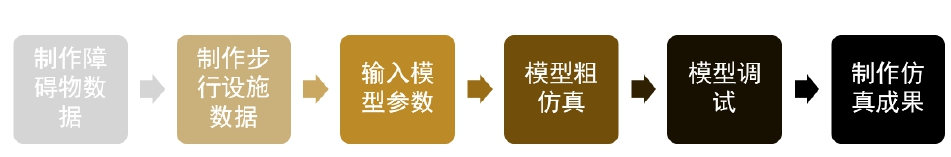
\includegraphics[width=\textwidth]{chp06_微观行人仿真模型的建模流程.jpg}
  \caption{微观行人仿真模型的建模流程\label{fig:chp06_微观行人仿真模型的建模流程} }
\end{figure}

\subsection{制作障碍物数据}
障碍物数据是以室内设计图为基础, 针对建筑内外墙体、 支撑结构、限制区
等行人无法通行的边界进行设定,保证仿真模型中的行人个体能够在有效的区域
进行活动, 不会超出仿真范围。 全部作业在 AutoCAD 软件中开展,最终的成果
是一个经过抽象后的线状边界文件,格式是 AutoCAD 软件支持的 dwg 格式。

\begin{figure}[!ht]
  \centering
  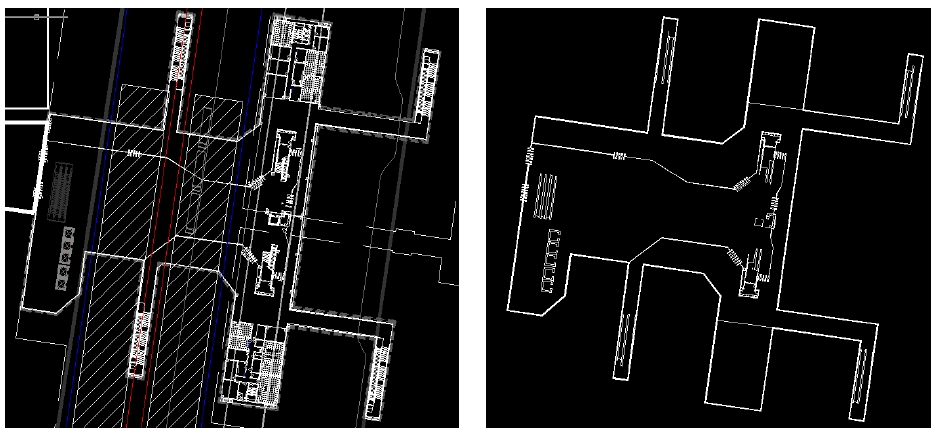
\includegraphics[width=\textwidth]{chp06_障碍物数据图纸.jpg}
  \caption[抽象出障碍物数据]{抽象出障碍物数据(左图是规划设计图纸, 右图是根据设计图中建筑和设施边界抽象出的障碍物数据)\label{fig:chp06_障碍物数据图纸} }
\end{figure}

\subsection{制作步行设施数据}
步行设施数据是指枢纽内部行人步行过程中会使用的室内设施, 比如电梯、
楼梯、闸机、 门、 列车等, 这些设施对行人的步行速度、 方式和空间都会有特定
的影响,因此需要区别于障碍物数据进行单独建模。 Legion 软件中针对这些特殊
的步行设施基本上都有相应的仿真模块。 例如,下图是手扶电梯模块, 包括进入
区、上升区、 离开区、 进入线、 离开线等实体, 而且在每个区域还可以设计特殊
的速度来模拟真实场景。

\begin{figure}[!ht]
  \centering
  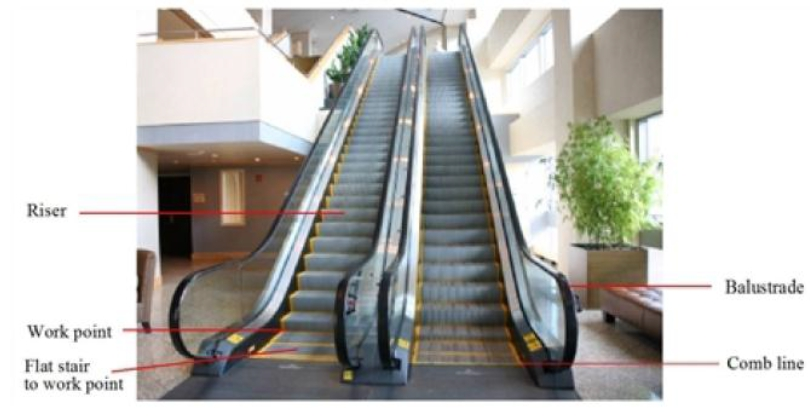
\includegraphics[width=\textwidth]{chp06_Legion行人仿真软件中的手扶电梯模块1.jpg} 
\end{figure}

\begin{figure}[!ht]
  \centering
  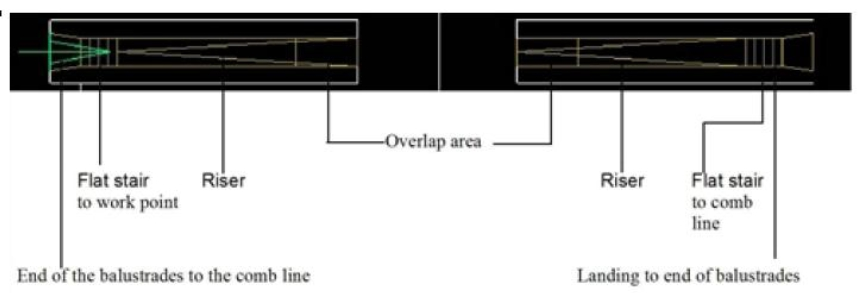
\includegraphics[width=\textwidth]{chp06_Legion行人仿真软件中的手扶电梯模块2.jpg}
  \caption{Legion行人仿真软件中的手扶电梯模块\label{fig:chp06_Legion行人仿真软件中的手扶电梯模块} }
\end{figure}

针对需要仿真的步行设施在 Legion 软件中进行实体建模,最终形成步行设
施数据,这部分数据与前面的障碍物数据一起构成了行人仿真模型的静态形状数据集。

\begin{figure}[!ht]
  \centering
  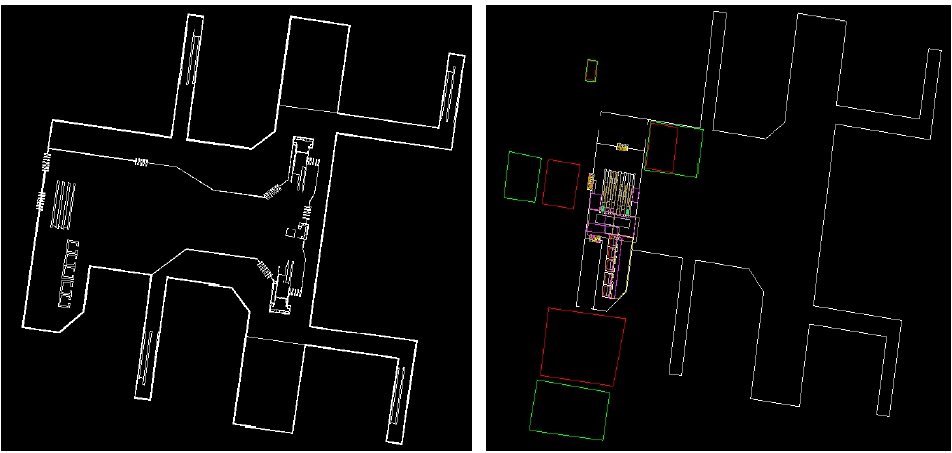
\includegraphics[width=\textwidth]{chp06_添加步行设施数据.jpg}
  \caption[添加步行设施数据]{添加步行设施数据。左图是障碍物数据,右图是添加了仿真模块的步行设施数据
\label{fig:chp06_添加步行设施数据} }
\end{figure}

\subsection{输入模型参数}
为了能够更加真实地对场景进行仿真, Legion 建模技术设计了一系列参数对
个体和流量特征进行模拟,其中重要的参数包括以下五类:

\begin{para}
\item[行人参数设置]包括行人的国籍、步行速度、身材、行李大小等
\item[行人类别设置]按照人群对个体进行分类,针对每类人群的组成和属性进行设置
\item[OD 需求设置]输入枢纽进出站的位置、区域以及 OD 人流量
\item[时间参数设置]设定每个进出站位置行人产生的概率密度分布、 行人排
队购票时间、 候车时间等参数
\item[其他设置]主要包括列车车厢的密度、列车发车间隔
\end{para}

所有的参数输入可以直接在 Legion 软件中完成,也可以在 Legion 软件专门
设计的一个 excel 文件中完成。 如果是初始输入,通常使用特定 excel 文件进行
输入, 可以比较方便的进行批量输入和修改;而针对局部参数的修改可以直接在
Legion 软件中完成。 图\ref{fig:Legion行人仿真参数输入中采用的特定excel文件结构}是特定 excel 文件中包含的五张工作簿。

\begin{figure}[!ht]
  \centering
  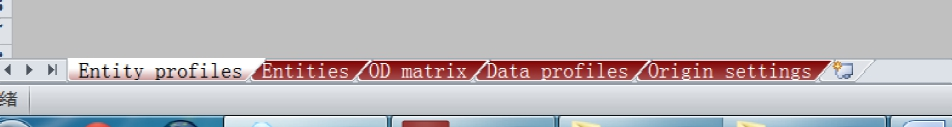
\includegraphics[width=0.7\textwidth]{chp06_Legion行人仿真参数输入中采用的特定excel文件结构.jpg}
  \caption{Legion行人仿真参数输入中采用的特定excel文件结构\label{fig:Legion行人仿真参数输入中采用的特定excel文件结构} }
\end{figure}

\subsection{模型粗仿真}
完成上述模型数据的输入之后,可以在 Legion 软件中运行模型, Legion 会
根据设定的参数对每个个体进行步行仿真,包括出发点、目的地、步行速度,并
且根据导航算法自动规划行人轨迹, 比如行人会具有优先选择最短的路径、 最不
拥堵的路径等行为, 最终得到模型粗仿真成果如下图所示。

\begin{figure}[!ht]
  \centering
  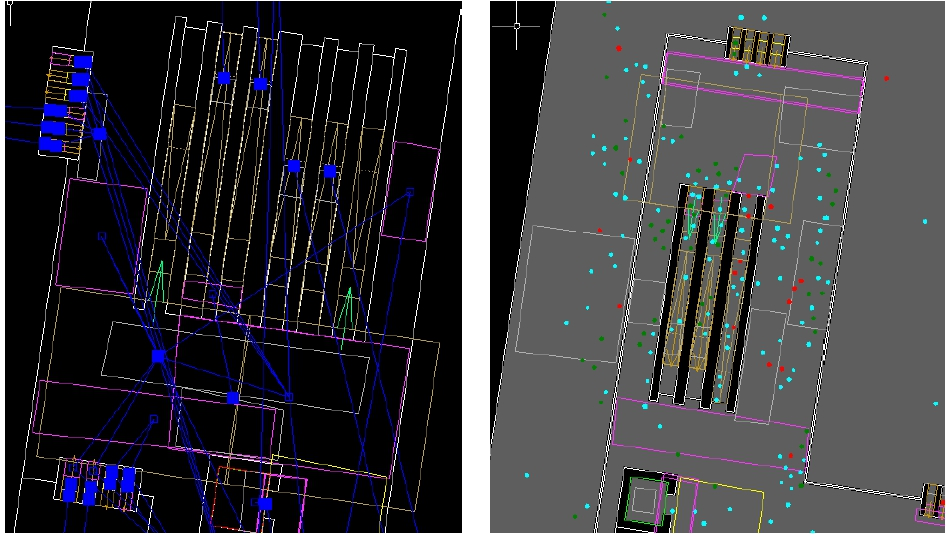
\includegraphics[width=0.9\textwidth]{chp06_行人仿真模型粗仿真成果.jpg}
  \caption{行人仿真模型粗仿真成果\label{fig:chp06_行人仿真模型粗仿真成果} }
\end{figure}

\subsection{模型调试}
虽然 Legion的自动导航算法能够给每个仿真个体设定一种通用的步行行为,
但是真实场景远比选择距离最短、最不拥堵这些简单规则要复杂, 因此在粗仿真
过程中会发现一些个体出现很异常的行为, 比如所有从特定出发点到目的地的个
体都选择相同的路径; 如果有手扶电梯和楼梯同时存在时, 无人使用楼梯等,这
些于真实场景都是有差异的。

Legion 软件中提供了对个体仿真过程中的查看机制,可以对每个时间切片的
个体行为进行观察,包括出发点、 最终目的地、 下一目的地、个体属性等。 利用
这项功能可以对异常个体进行追踪, 观察其仿真过程中的行为, 分析异常情况产
生的原因,然后在根据实际情况和具体方案进行模型参数调试,从而使模型能够
更好地模拟真实场景。

\begin{figure}[!ht]
  \centering
  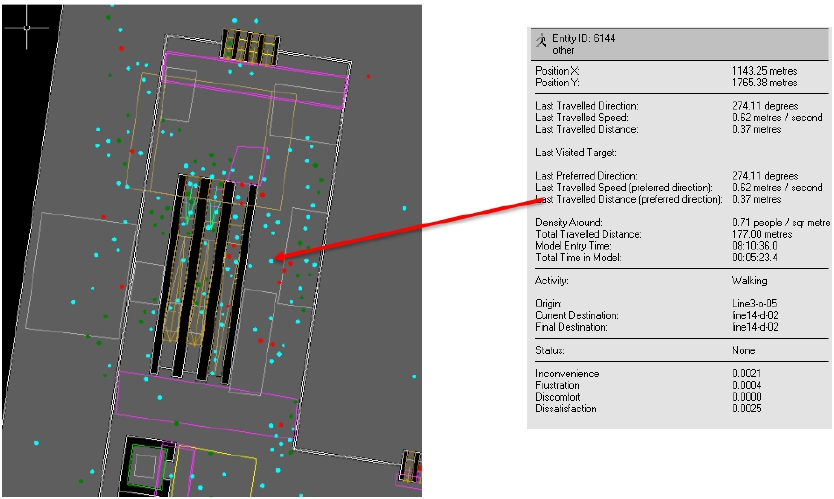
\includegraphics[width=0.9\textwidth]{chp06_Legion软件中的个体查看功能.jpg}
  \caption{Legion软件中的个体查看功能\label{fig:chp06_Legion软件中的个体查看功能} }
\end{figure}

\section{大运枢纽站行人仿真成果}
行人仿真最终成果包括视频录像和数据分析图。其中视频录像可以比较直观
地观察行人在二维平面上的运动, 用动画的形式分析单个潜在拥堵形成的过程。
数据分析图则对某个时间切片的人流量数据进行分析, 可以以密度分析图的形式
展现人流密度的空间分布, 从而对枢纽行人组织方案进行全局判断和评估。

图\ref{fig:chp06_大运枢纽地上二层行人仿真视频录像截图}是大运枢纽站地上二层的仿真视频录像截图, 视频文件可以在项目成果文件夹中进行查看。图\ref{fig:chp06_大运枢纽行人仿真成果密度分析图}是每层行人仿真成果的密度颜色图。

\begin{figure}[!ht]
  \centering
  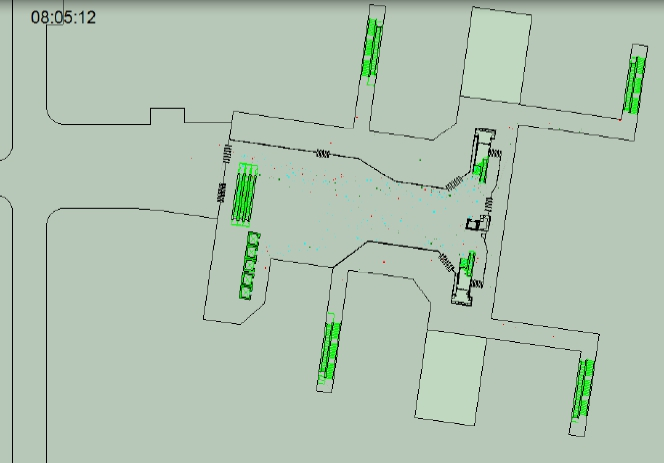
\includegraphics[width=0.9\textwidth]{chp06_大运枢纽地上二层行人仿真视频录像截图.jpg}
  \caption{大运枢纽地上二层行人仿真视频录像截图\label{fig:chp06_大运枢纽地上二层行人仿真视频录像截图} }
\end{figure}

\begin{figure}[!ht]
  \centering
  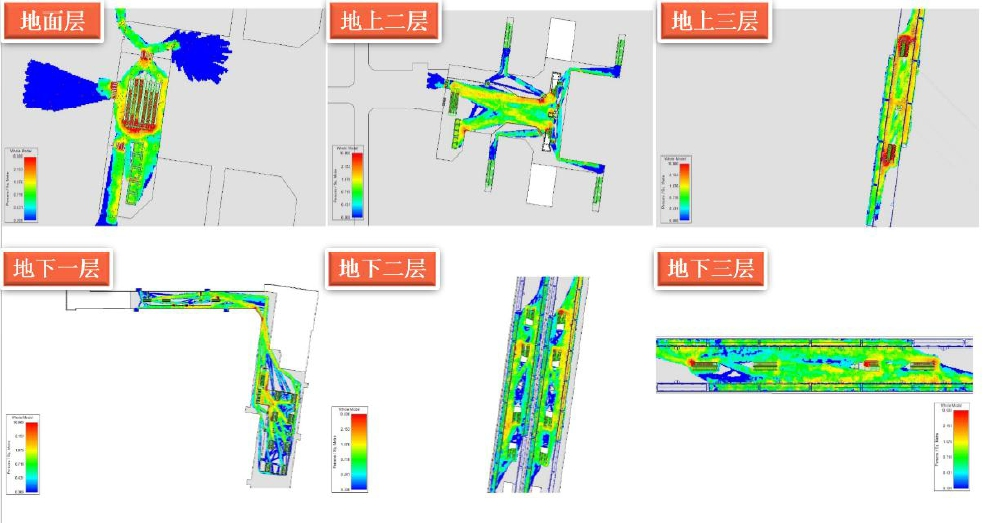
\includegraphics[width=\textwidth]{chp06_大运枢纽行人仿真成果密度分析图.jpg}
  \caption{大运枢纽行人仿真成果密度分析图\label{fig:chp06_大运枢纽行人仿真成果密度分析图} }
\end{figure}

\section{高新园站行人仿真成果}
高新园站行人仿真最终成果为数据分析图,如图\ref{fig:chp06_高新园站行人仿真成果密度分析图}所示。

\begin{figure}[!ht]
  \centering
  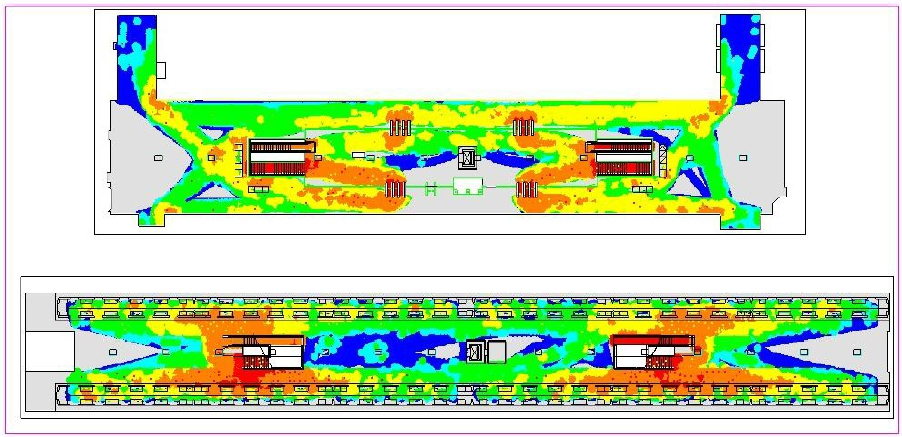
\includegraphics[width=\textwidth]{chp06_高新园站行人仿真成果密度分析图.jpg}
  \caption{高新园站行人仿真成果密度分析图\label{fig:chp06_高新园站行人仿真成果密度分析图} }
\end{figure}




